\documentclass{article}
\usepackage[T1]{fontenc}
\usepackage{lmodern}
\usepackage{graphicx}
\usepackage{amsmath,amssymb}
\usepackage[a4paper,margin=2cm]{geometry}
\usepackage[absolute,overlay]{textpos}
\setlength{\TPHorizModule}{1mm}
\setlength{\TPVertModule}{1mm}
\usepackage[indonesian]{babel}
\usepackage{hyperref}
\setlength{\emergencystretch}{2em}
% unit: Halaman 47

\begin{document}

% === Halaman 47 (llm) ===

\section*{Double DES}

\vspace{89.10mm}

\begin{itemize}
    \item Menggunakan 2 buah kunci eksternal, $K_1$ dan $K_2$.
    \item Enkripsi: \[ C = E_{K_2}(E_{K_1}(P)) \]
    \item Dekripsi: \[ P = D_{K_1}(D_{K_2}(C)) \]
\end{itemize}

\vspace{30mm}

\vspace{30mm}

% deskripsi: Diagram alir proses enkripsi Double DES yang menunjukkan plaintext P melewati dua tahap enkripsi (E) menggunakan kunci K1 dan K2 untuk menghasilkan ciphertext C.
% bbox normalisasi: [0.3950, 0.2700, 0.8300, 0.5700]
\begin{textblock*}{91.35mm}(82.95mm,80.19mm)
\noindent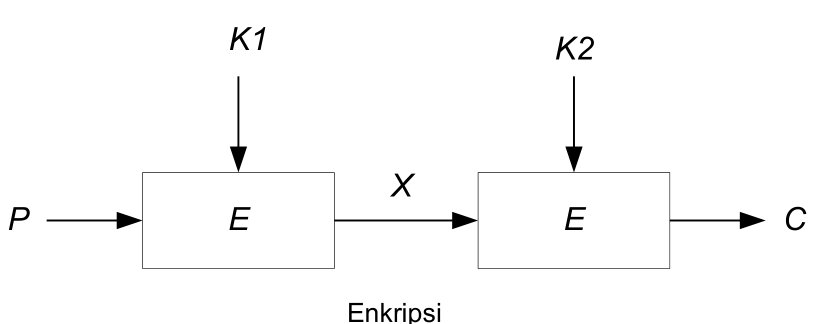
\includegraphics[width=91.35mm,height=89.10mm]{../../images/llm/page_047_img_01.png}%
\end{textblock*}

% deskripsi: Diagram alir proses dekripsi Double DES yang menunjukkan ciphertext C melewati dua tahap dekripsi (D) menggunakan kunci K2 dan K1 untuk menghasilkan plaintext P.
% bbox normalisasi: [0.3950, 0.6200, 0.8300, 0.9000]
\begin{textblock*}{91.35mm}(82.95mm,184.14mm)
\noindent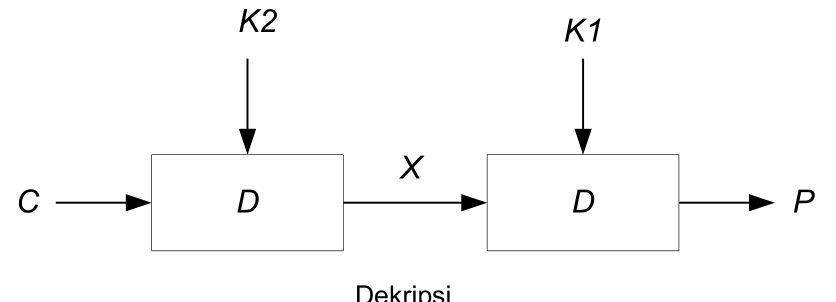
\includegraphics[width=91.35mm,height=83.16mm]{../../images/llm/page_047_img_02.png}%
\end{textblock*}

\end{document}
